% Credits are indicated where needed. The general idea is based on a template by Vel (vel@LaTeXTemplates.com) and Frits Wenneker.

\documentclass[11pt, a4paper]{article} % General settings in the beginning (defines the document class of your paper)
% 11pt = is the font size
% A4 is the paper size
% “article” is your document class

%----------------------------------------------------------------------------------------
%	Packages
%----------------------------------------------------------------------------------------

% Necessary
\usepackage[german,english]{babel} % English and German language 
\usepackage{booktabs} % Horizontal rules in tables 
% For generating tables, use “LaTeX” online generator (https://www.tablesgenerator.com)
\usepackage{placeins}
\usepackage{comment} % Necessary to comment several paragraphs at once
\usepackage[utf8]{inputenc} % Required for international characters
\usepackage[T1]{fontenc} % Required for output font encoding for international characters

% Might be helpful
\usepackage{amsmath,amsfonts,amsthm} % Math packages which might be useful for equations
\usepackage{tikz} % For tikz figures (to draw arrow diagrams, see a guide how to use them)
\usepackage{tikz-cd}
\usetikzlibrary{positioning,arrows} % Adding libraries for arrows
\usetikzlibrary{decorations.pathreplacing} % Adding libraries for decorations and paths
\usepackage{tikzsymbols} % For amazing symbols ;) https://mirror.hmc.edu/ctan/graphics/pgf/contrib/tikzsymbols/tikzsymbols.pdf 
\usepackage{blindtext} % To add some blind text in your paper


%---------------------------------------------------------------------------------
% Additional settings
%---------------------------------------------------------------------------------
\usepackage{indentfirst} 
%---------------------------------------------------------------------------------
% Define your margins
\usepackage{geometry} % Necessary package for defining margins

\geometry{
	top=2cm, % Defines top margin
	bottom=2cm, % Defines bottom margin
	left=2.2cm, % Defines left margin
	right=2.2cm, % Defines right margin
	includehead, % Includes space for a header
	%includefoot, % Includes space for a footer
	%showframe, % Uncomment if you want to show how it looks on the page 
}

\setlength{\parindent}{15pt} % Adjust to set you indent globally 

%---------------------------------------------------------------------------------
% Define your spacing
\usepackage{setspace} % Required for spacing
% Two options:
\linespread{1.5}
%\onehalfspacing % one-half-spacing linespread

%----------------------------------------------------------------------------------------
% Define your fonts
\usepackage[T1]{fontenc} % Output font encoding for international characters
\usepackage[utf8]{inputenc} % Required for inputting international characters

\usepackage{XCharter} % Use the XCharter font


%---------------------------------------------------------------------------------
% Define your headers and footers

\usepackage{fancyhdr} % Package is needed to define header and footer
\pagestyle{fancy} % Allows you to customize the headers and footers
\setlength{\headheight}{13.59999pt} % Adjust head height to avoid fancyhdr warning

%\renewcommand{\sectionmark}[1]{\markboth{#1}{}} % Removes the section number from the header when \leftmark is used

% Headers
\lhead{STAT 333} % Define left header
\chead{\textit{}} % Define center header - e.g. add your paper title
\rhead{Regression Runner} % Define right header

% Footers
\lfoot{} % Define left footer
\cfoot{\footnotesize \thepage} % Define center footer
\rfoot{ } % Define right footer

%---------------------------------------------------------------------------------
%	Add information on bibliography
\usepackage{natbib} % Use natbib for citing
\usepackage{har2nat} % Allows to use harvard package with natbib https://mirror.reismil.ch/CTAN/macros/latex/contrib/har2nat/har2nat.pdf

% For citing with natbib, you may want to use this reference sheet: 
% http://merkel.texture.rocks/Latex/natbib.php

%---------------------------------------------------------------------------------
% Add field for signature (Reference: https://tex.stackexchange.com/questions/35942/how-to-create-a-signature-date-page)
\newcommand{\signature}[2][5cm]{%
  \begin{tabular}{@{}p{#1}@{}}
    #2 \\[2\normalbaselineskip] \hrule \\[0pt]
    {\small \textit{Signature}} \\[2\normalbaselineskip] \hrule \\[0pt]
    {\small \textit{Place, Date}}
  \end{tabular}
}
%---------------------------------------------------------------------------------
%	General information
%---------------------------------------------------------------------------------
\title{title} % Adds your title
\author{
Stanley Zheng \space Eric \space Lucas
% Add your first and last name
    \thanks{Equal contribution} % Adds a footnote to your title
    %\institution{YOUR INSTITUTION} % Adds your institution
  }

\date{\small \today} % Adds the current date to your “cover” page; leave empty if you do not want to add a date


%---------------------------------------------------------------------------------
%	Define what’s in your document
%---------------------------------------------------------------------------------

\begin{document}


% If you want a cover page, uncomment "\input{coverpage.tex}" and uncomment "\begin{comment}" and "\end{comment}" to comment the following lines
%\input{coverpage.tex}

%\begin{comment}
\maketitle % Print your title, author name and date; comment if you want a cover page 

% \begin{center} % Center text
%     Word count: XXXX
% % How to check words in a LaTeX document: https://www.overleaf.com/help/85-is-there-a-way-to-run-a-word-count-that-doesnt-include-latex-commands
% \end{center}
%\end{comment}

%----------------------------------------------------------------------------------------
% Abstract
%----------------------------------------------------------------------------------------
\setcounter{page}{1} % Sets counter of page to 1
%----------------------------------------------------------------------------------------
% Introduction
%----------------------------------------------------------------------------------------

\section{Introduction} % Main section title

\subsection{Motivation: The Shifting Landscape of the NBA} % Sub-section 1.1
% Paragraph 1: General observation and the basic rule
Over the last couple of decades, anyone watching the NBA has noticed a big change in how the game is played. We see teams shooting way more three-pointers than before. It makes sense to ask why. In the NBA, the basic rule is that shots made inside the arc are worth 2 points, while shots made further out, behind the arc, are worth 3 points. This simple difference in scoring value seems to have encouraged teams to focus more and more on shooting from distance.

% Paragraph 2: The "Three-Point Era" narrative and motivation for study
This trend is so noticeable that people often talk about the modern NBA as the "Three-Point Era." Famous players like Stephen Curry really showed how valuable long-range shooting can be, making teams rethink their strategies. But is this just a popular trend, or has the actual importance of making three-pointers for winning games really increased compared to the past? For teams trying to win championships, understanding if and how the value of different shots has changed is really important. In today's world with lots of data available, we felt that using statistical analysis could help quantify this change and maybe offer useful insights for teams trying to optimize how they play.

\subsection{Research Question and Approach} % Sub-section 1.2
% Paragraph 1: Core question and the "story"

So, the main question we wanted to investigate in this project is: How has the *statistical association* between key shooting metrics, especially three-point percentage (3P\%), and team success, measured by win rate, changed over the last approximately 15-20 years? Our "story" is essentially testing the common idea that the NBA has truly entered a "three-point era" where making threes is more strongly linked to winning than it used to be.

% Paragraph 2: Challenge and approach
We need to be careful, though. We are using data collected from watching games (observational data), not from a controlled experiment like an RCT (Randomized Controlled Trial). This means we can't easily prove that shooting more threes *causes* more wins, because many other things might be happening at the same time (like better players, different defenses, rule changes). So, our approach is to use statistical tools, mainly multiple linear regression, and specifically interaction terms. These tools allow us to look for strong patterns or *structural evidence* in the data that show if the association between 3P\% and winning has really changed significantly over time, while trying to account for some other factors. Our goal is to describe this change accurately based on the statistics, aiming for an interpretation that acknowledges these limitations but points towards the changing dynamics (a quasi-causal goal).

\subsection{Thesis Statement} % Sub-section 1.3
% Paragraph 1: Presenting the thesis
Using data from the 2005-2009 and 2020-2024 NBA regular seasons (source: NBA API), we find the statistical association between three-point percentage (3P\%) and win rate differs significantly between these periods: NBA team-seasons (unit of analysis) in the 2020-2024 period with higher 3P\% also have statistically significant higher win rates, while NBA team-seasons in the 2005-2009 period did not have statistically significant higher win rates, even after controlling for two-point efficiency and shot selection proportions.

\subsection{Report Outline} % Sub-section 1.4 (Optional but recommended)
% Paragraph 1: Roadmap
The remainder of this report details the methodology we used, including data sources, variable definitions, and statistical techniques. We then present the results, including descriptive visualizations and the findings from our regression models. Finally, we conclude by discussing the implications of our results in relation to our thesis statement and acknowledging the limitations of our study.

%----------------------------------------------------------------------------------------
% End of Introduction Section
%----------------------------------------------------------------------------------------

%----------------------------------------------------------------------------------------
% Data Analysis
%----------------------------------------------------------------------------------------

\section{Data Analysis}
\subsection{Data Preprocess}
Our data preprocessing involved three major steps. First, we retrieved the raw data from an API, where each table corresponds 
to a different season, and each row records a team's performance for that year. Therefore, our unit of analysis is team/year.

As shown in Figure \ref{fig:original_data}, a large portion of the raw variables consisted of rankings (e.g., team rank in various metrics), 
which we decided to remove, as they are not suitable for our analysis. We also observed that the raw data already included some 
basic performance statistics, such as win percentage (W\_PCT) and three-point shooting percentage(FG3\_PCT). However, since the available 
statistics were limited to only a few dimensions, we manually calculated additional variables: win rate(WinRate), three-point attempt rate(3P\_ratio), 
three-point shooting percentage(3P\%), and two-point shooting percentage(2P\%).

We found that the three-point attempt rate and the two-point attempt rate are in a perfect linear relationship (they add up to 1), 
so we included only the three-point attempt rate in our models to avoid multicollinearity.

Finally, because most of our key variables, such as win rate and shooting percentages, naturally fall within the range [0, 1], 
we applied normalization to the other numerical variables as well to ensure these variables also fall with in the range [0, 1], 
which maintains the consistency across features. 

\subsection{Data Visulization}
To motivate our investigation into the evolving impact of three-point shooting on team success, we first examine two sets of histograms 
comparing the 2005-2009 and 2020-2024 NBA regular seasons.

The first set of histograms(Figure \ref{fig:3P_shooting_percent}) shows the three-point shooting percentage (3P\%), capturing efficiency on three-point attempts. While the 
distributions for the two periods overlap significantly, there is a modest rightward shift, indicating that teams have become slightly 
more accurate from beyond the arc over time. This suggests that the increase in three-point volume has not come at the expense of efficiency, 
but rather, teams have adapted by developing better shooters and improving shot quality.

\begin{figure}[htbp]
    \centering
    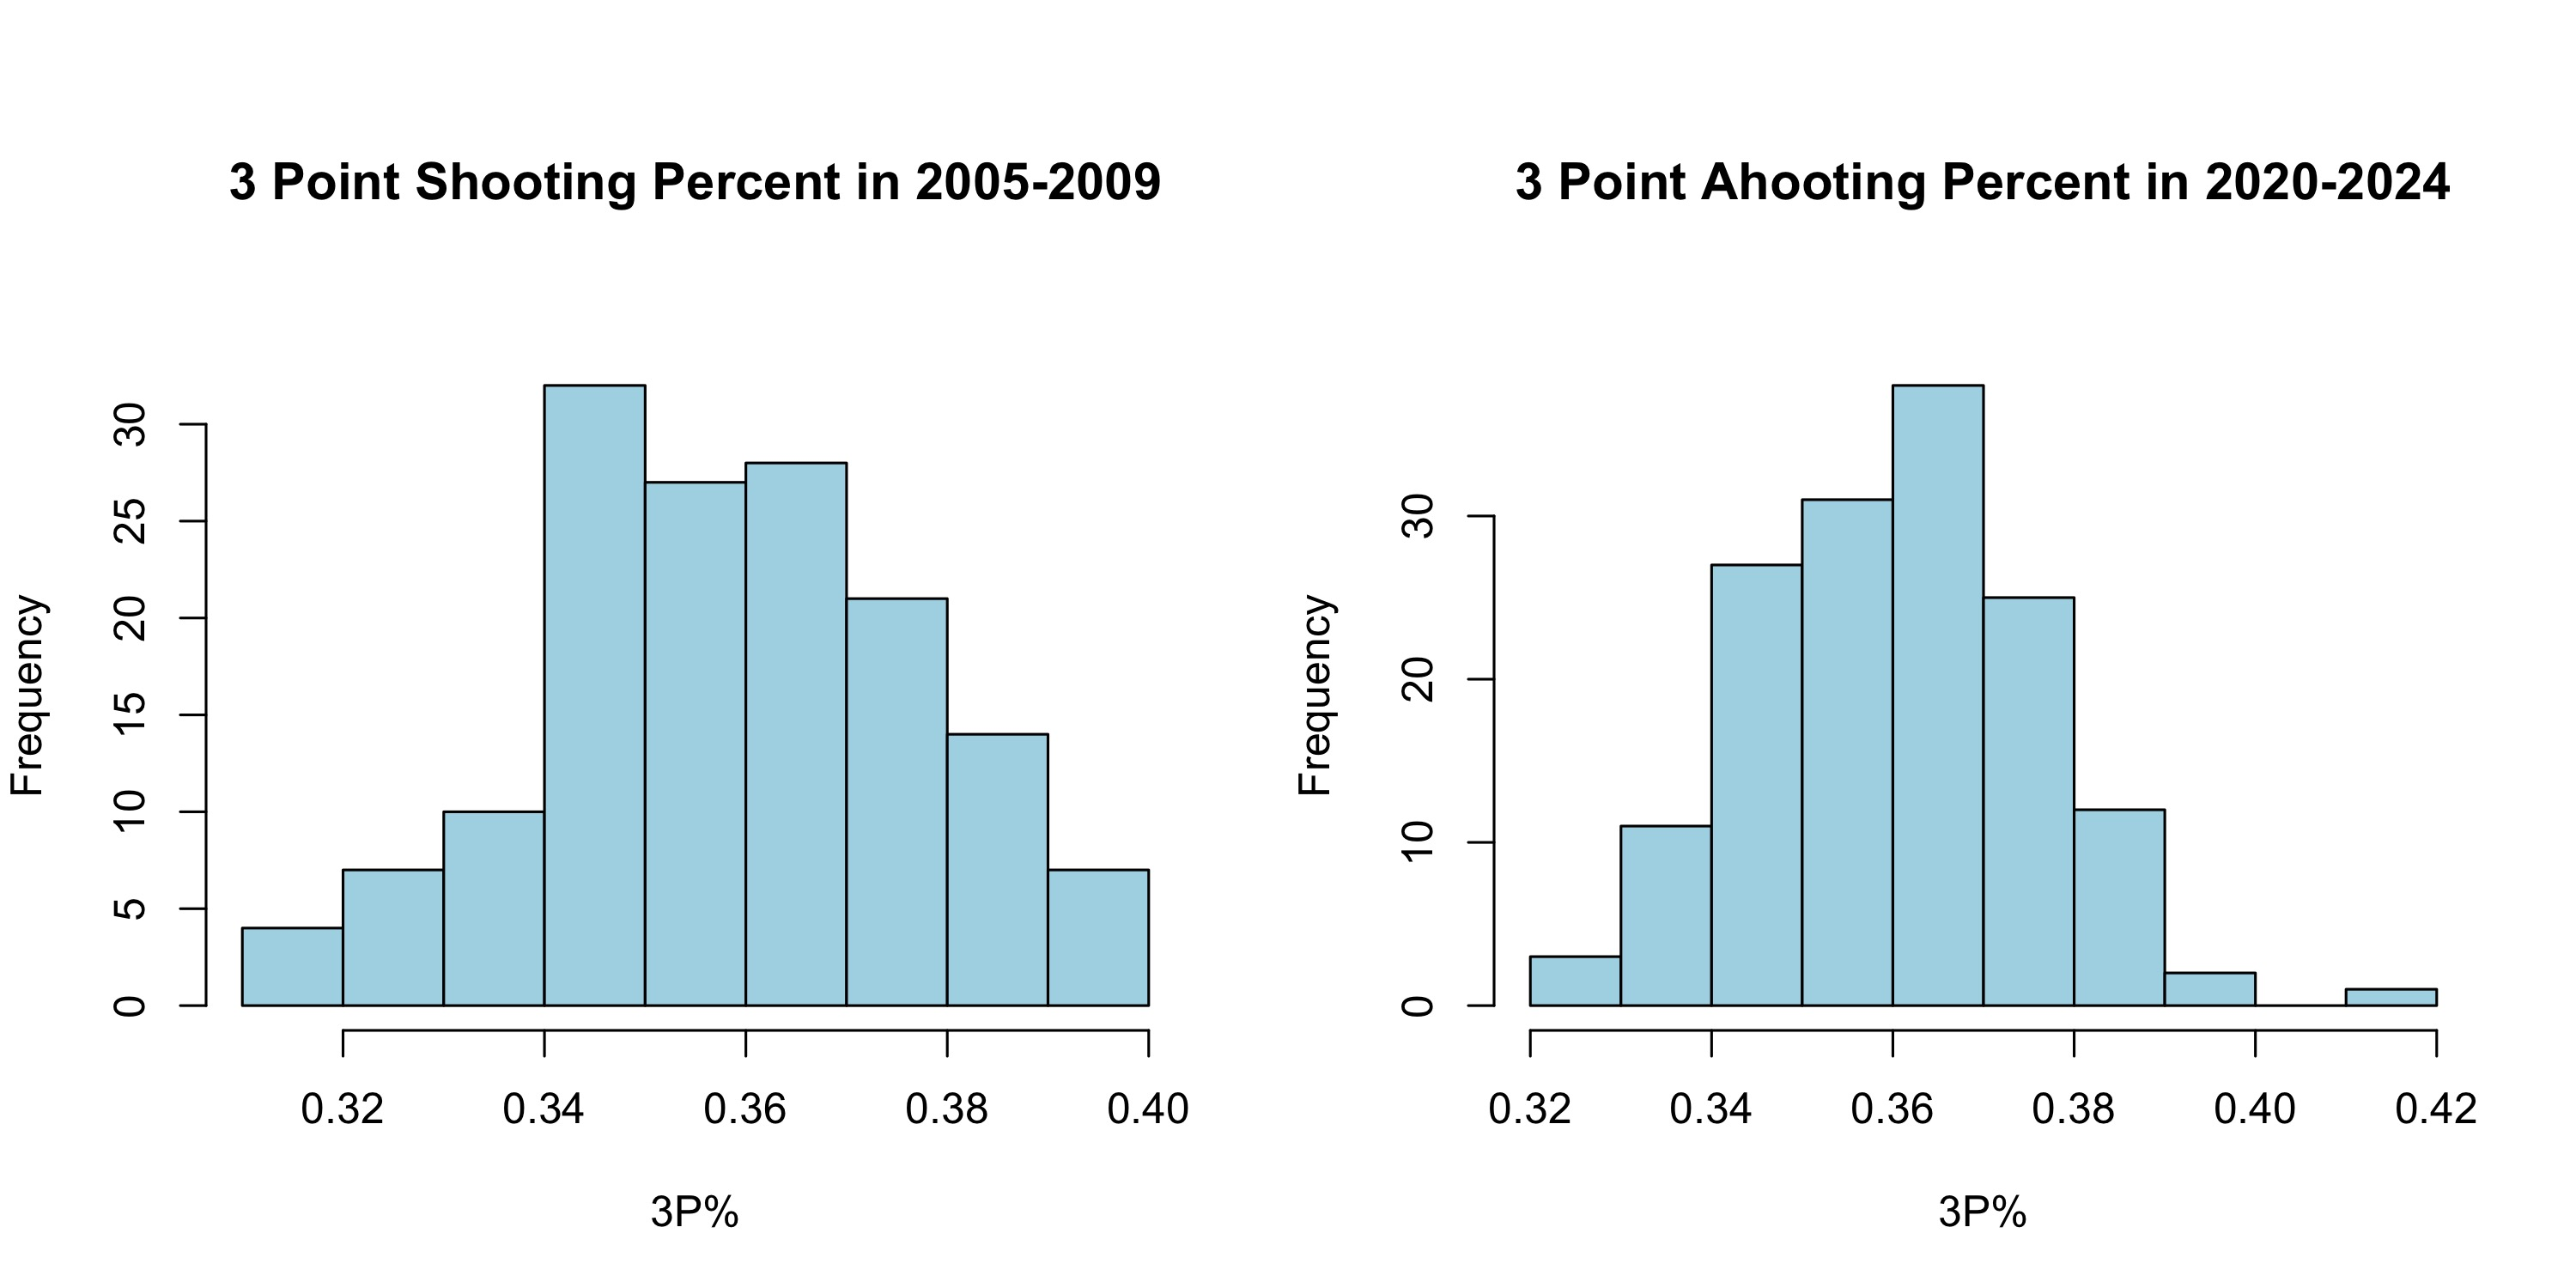
\includegraphics[width=0.9\textwidth]{figure/3P shooting percent.jpg}
    \caption{3 Point Shooting Percent in Two Different Period.}
    \label{fig:3P_shooting_percent}
\end{figure}

The second set of histograms(Figure \ref{fig:3P_attempt_rate}) displays the three-point attempt rate (3P\_ratio), defined as the proportion of a team's total field goal 
attempts that are three-pointers. We observe a substantial rightward shift over time: in the 2005–2009 period, teams clustered around a 
20\% attempt rate, whereas by 2020-2024, the distribution centers around 38-40\%. This sharp increase visually confirms the commonly 
cited notion that the NBA has entered a “small ball” era, characterized by greater reliance on perimeter shooting and faster-paced offenses.

\begin{figure}[htbp]
    \centering
    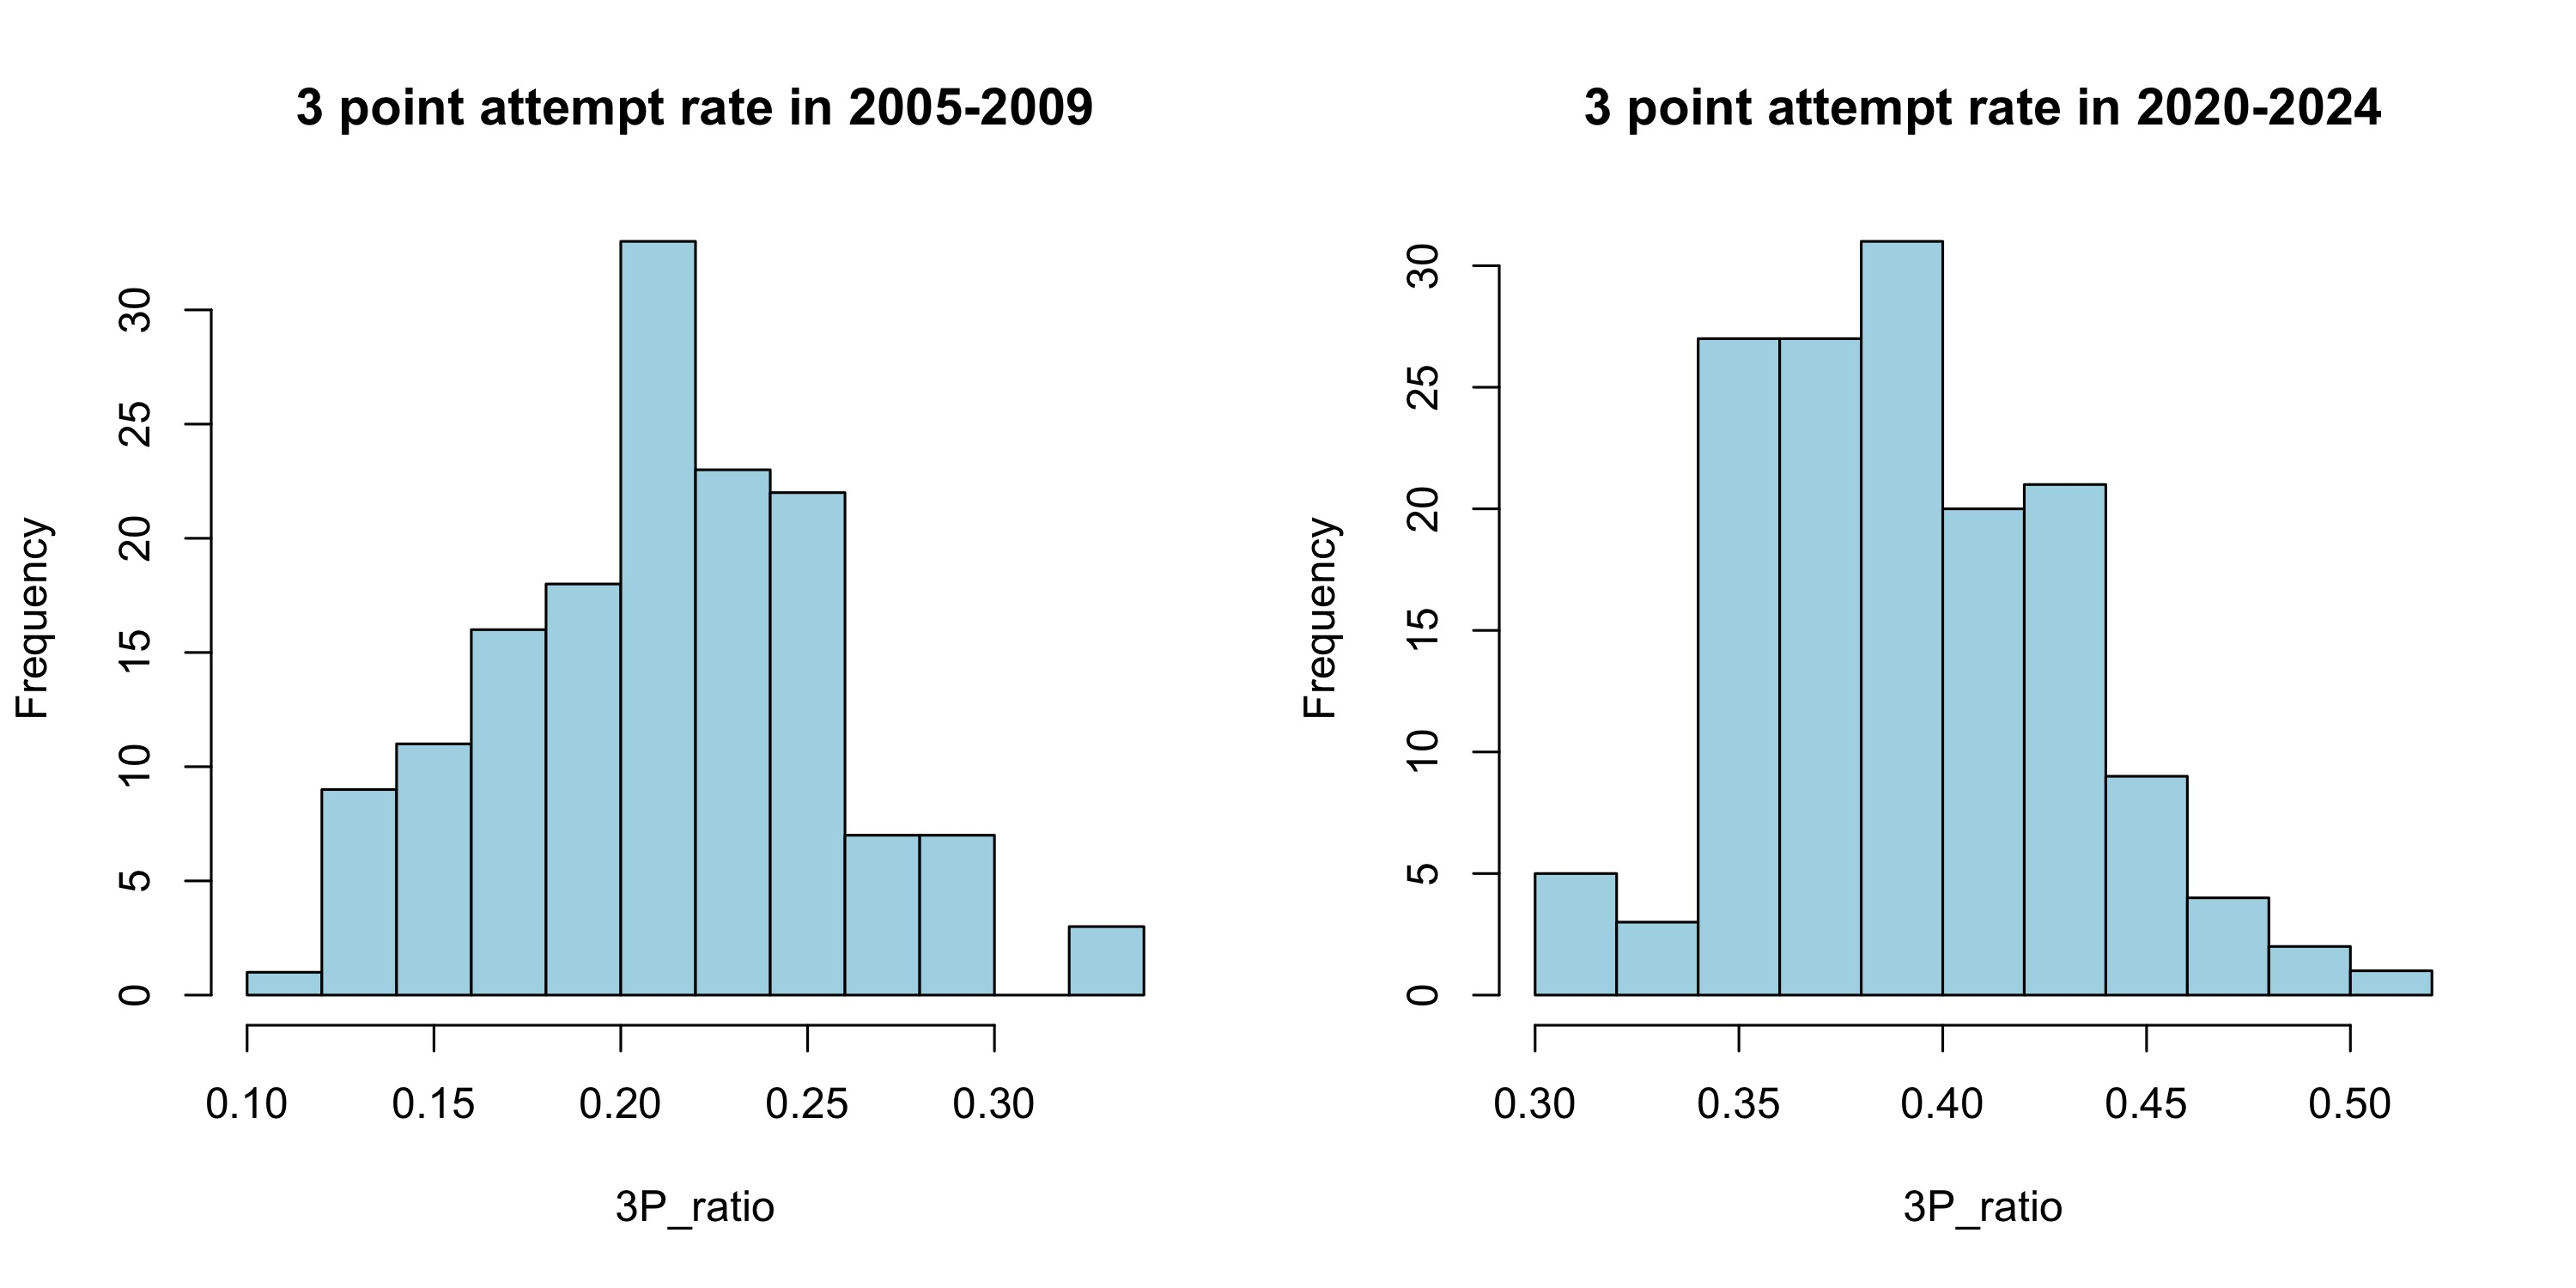
\includegraphics[width=0.9\textwidth]{figure/3 point attempt rate.jpg}
    \caption{3 Point Attempt Rate in Two Different Period.}
    \label{fig:3P_attempt_rate}
\end{figure}

Together, these visualizations provide structural evidence for a fundamental change in league-wide offensive strategy. 
The sharp increase in three-point attempt rates, coupled with stable or slightly improved three-point accuracy, sets the stage for our 
central analysis: evaluating whether and how the growing emphasis on three-point shooting translates into higher win rates in the modern NBA.


%----------------------------------------------------------------------------------------
% Results Section
%----------------------------------------------------------------------------------------

\section{Results}

This section presents the results of our data analysis. We first explore descriptive trends in shooting strategy and efficiency over time using visualizations. Then, we present the findings from our main statistical analysis using an interaction model to formally test our hypothesis about the changing association between three-point shooting and team success. Finally, we assess the validity of our chosen model through diagnostic checks.

\subsection{Descriptive Trends in Shooting Strategy and Efficiency}
% Word Count: Approx. 350-450 words

% Discuss Histograms
To understand the context of our analysis, we first visualized how shooting patterns have changed between the earlier period (2005-2009) and the more recent period (2020-2024), based on our aggregated datasets. Figure \ref{fig:3P_shooting_percent} compares the distribution of team three-point shooting percentages (3P\%) across these two eras. We observe some overlap, but also a slight shift to the right in the 2020-2024 period, suggesting a modest improvement or stability in average team three-point accuracy over time, even as attempt rates increased.

% Note: Ensure figure path 'figure/3P_shooting_percent.jpg' is correct
\begin{figure}[htbp]
    \centering
    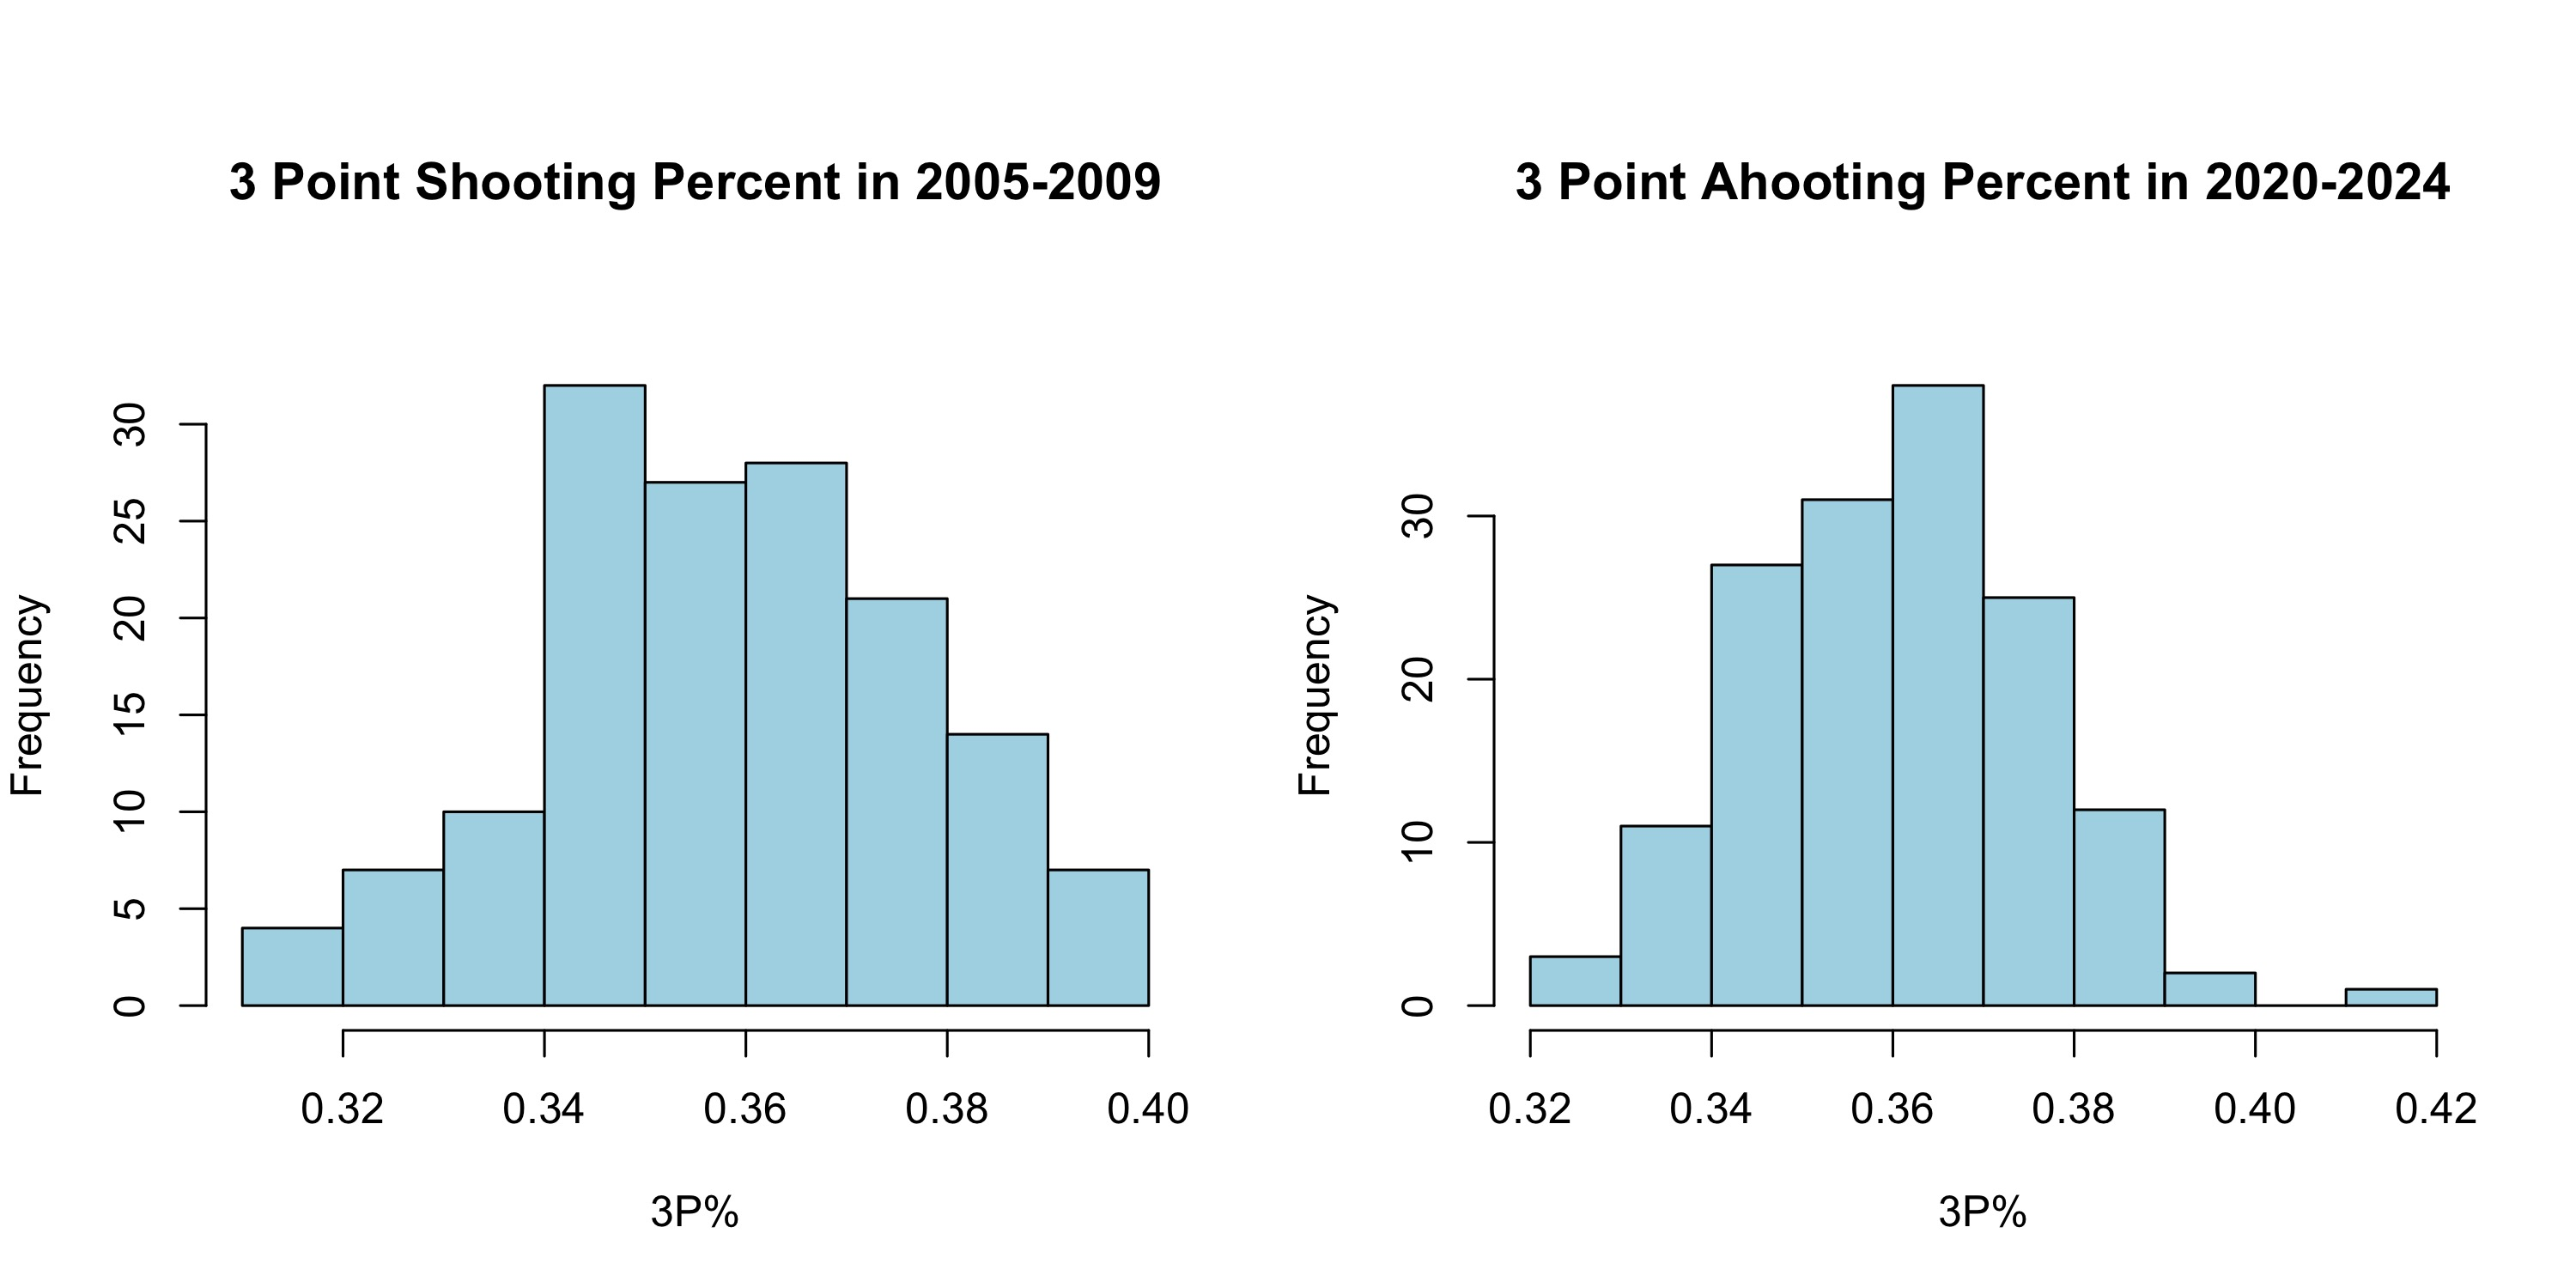
\includegraphics[width=0.9\textwidth]{figure/3P shooting percent.jpg} 
    \caption{Comparison of Team 3-Point Shooting Percentage (3P\%) Distributions: 2005-2009 vs. 2020-2024.}
    \label{fig:3P_shooting_percent}
\end{figure}

Figure \ref{fig:3P_attempt_rate} displays the distribution of the three-point attempt rate (3P\_ratio). The change here is striking. In 2005-2009, the distribution centered around 20\% of total shots being threes. By 2020-2024, this distribution clearly shifted, centering around 38-40\%. This visually confirms the dramatic increase in reliance on the three-point shot, characteristic of the "Three-Point Era".

\begin{figure}[htbp]
    \centering
    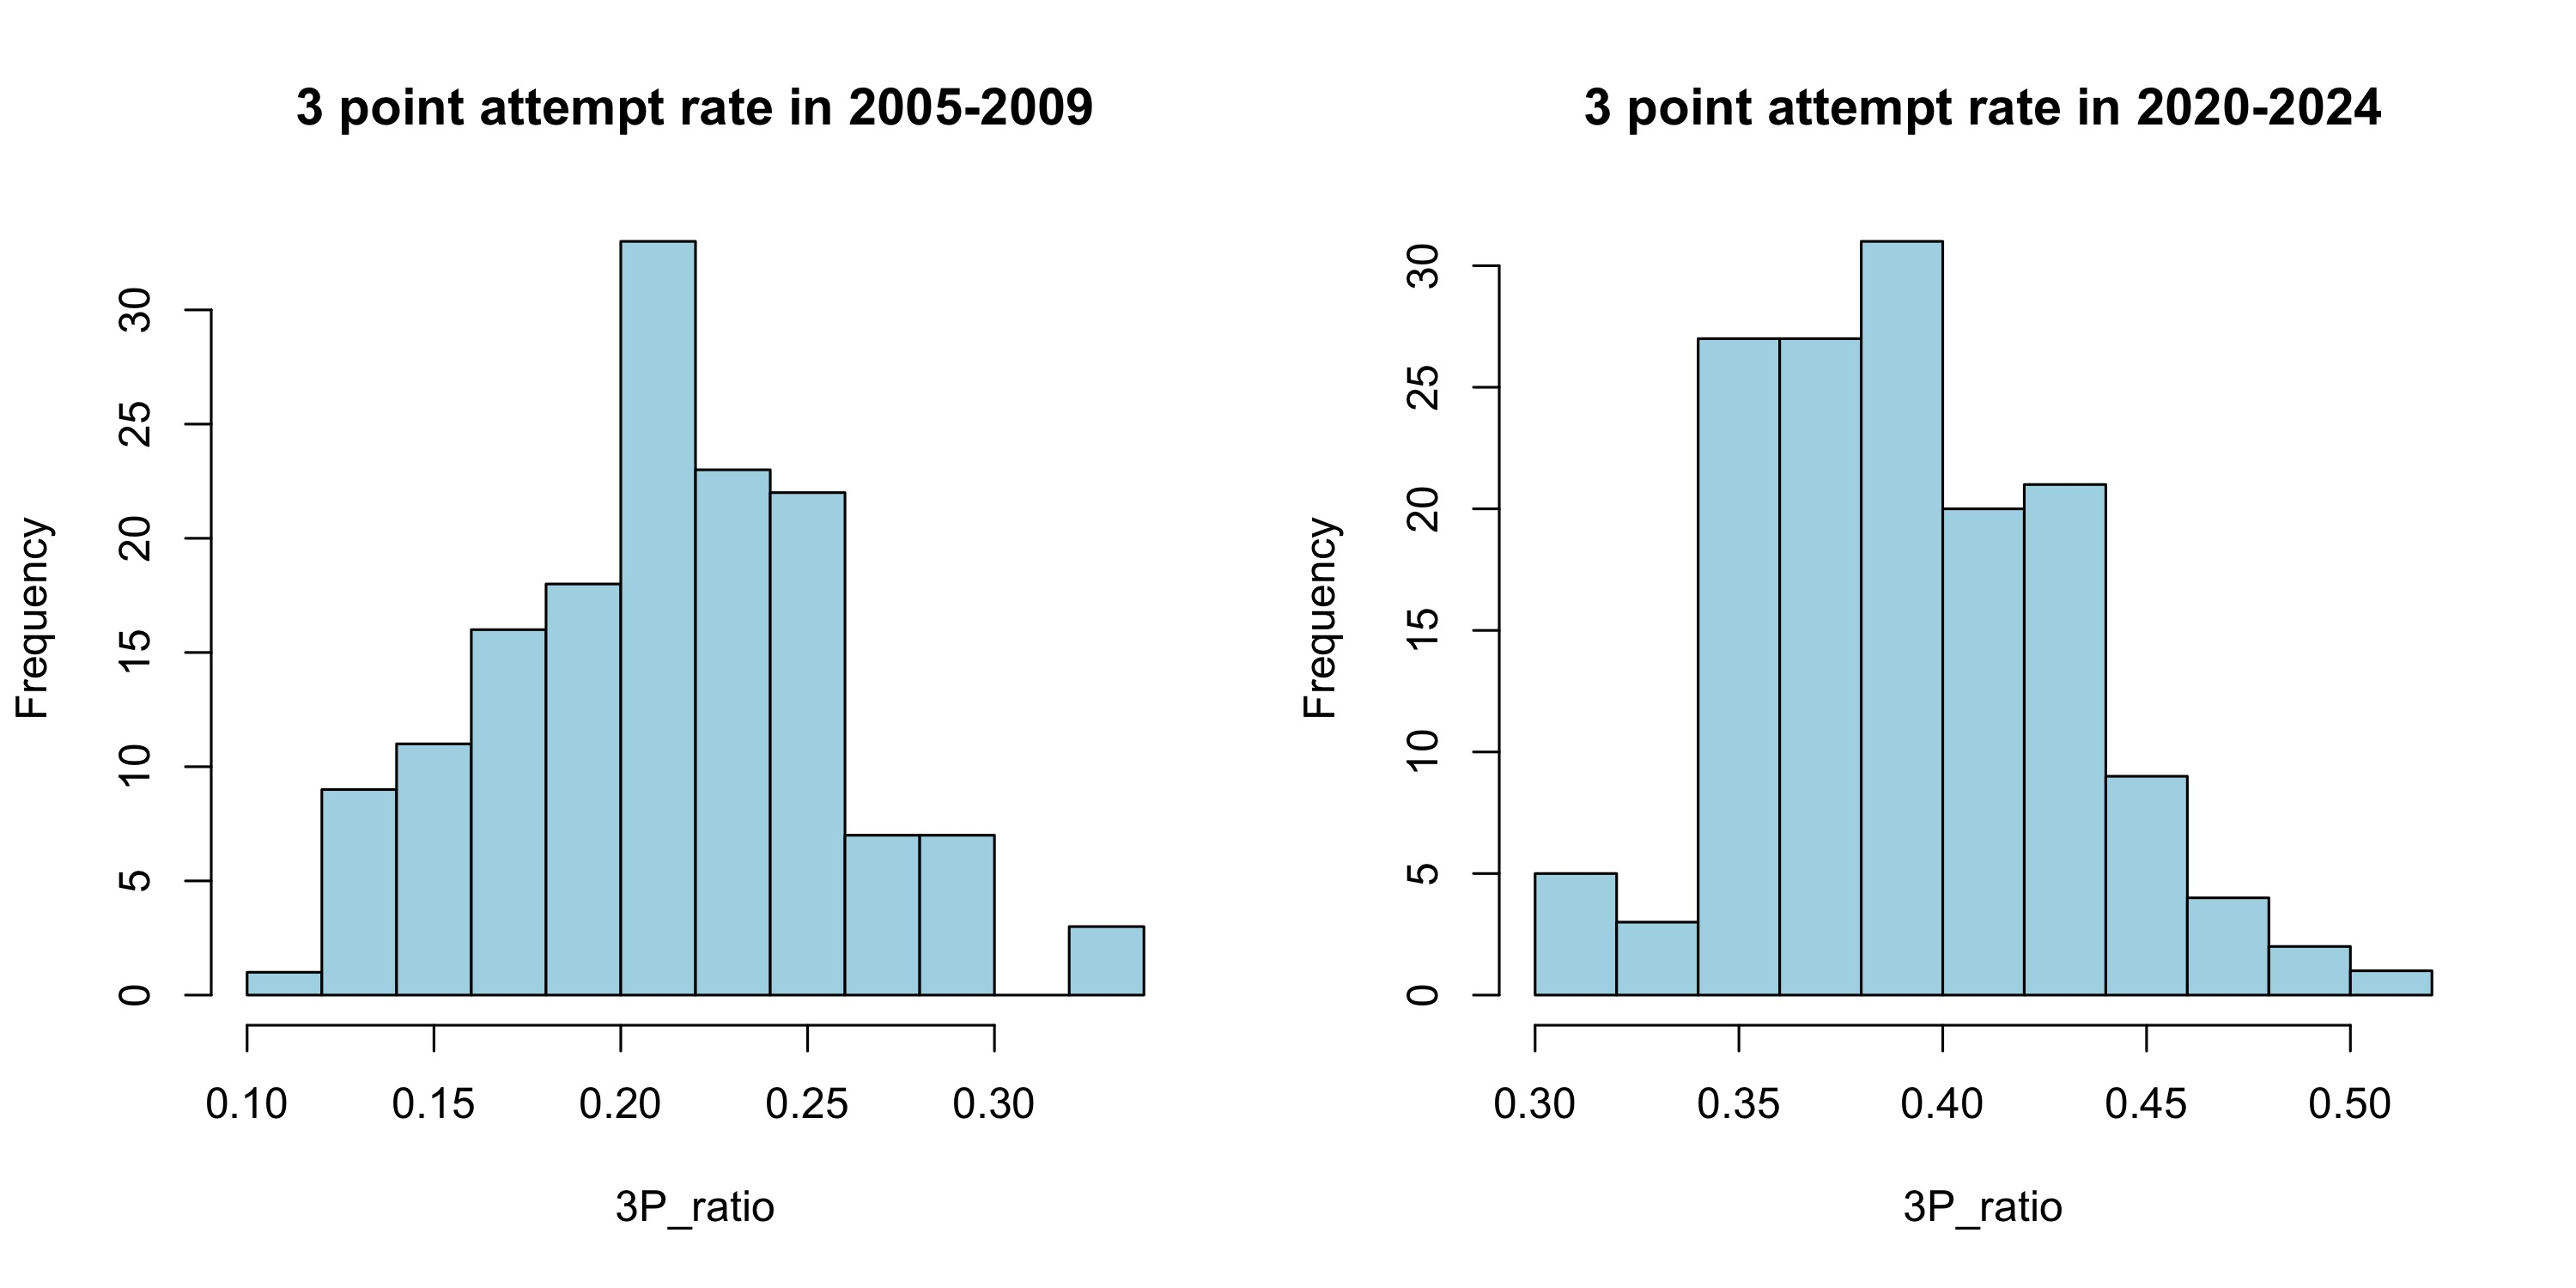
\includegraphics[width=0.9\textwidth]{figure/3 point attempt rate.jpg} 
    \caption{Comparison of Team 3-Point Attempt Rate (3P\_ratio) Distributions: 2005-2009 vs. 2020-2024.}
    \label{fig:3P_attempt_rate}
\end{figure}
\FloatBarrier
% Discuss Trend Plots
To visualize how the statistical association between shooting efficiency and winning might have evolved, we examined coefficients from separate regressions run on consecutive 5-year periods. Figure \ref{fig:coefficients_trends} plots the estimated coefficients for 3P\% and 2P\% over time. The plot reveals diverging trends: the coefficient associated with 3P\% (blue line) consistently increases across the periods, suggesting a strengthening positive association with win rate. In contrast, the coefficient associated with 2P\% (red line) shows a decreasing trend, suggesting that its association might weaken relative to 3P\%. This visual evidence strongly suggests a dynamical change and motivates the formal test using an interaction model.

\begin{figure}[htbp]
    \centering
    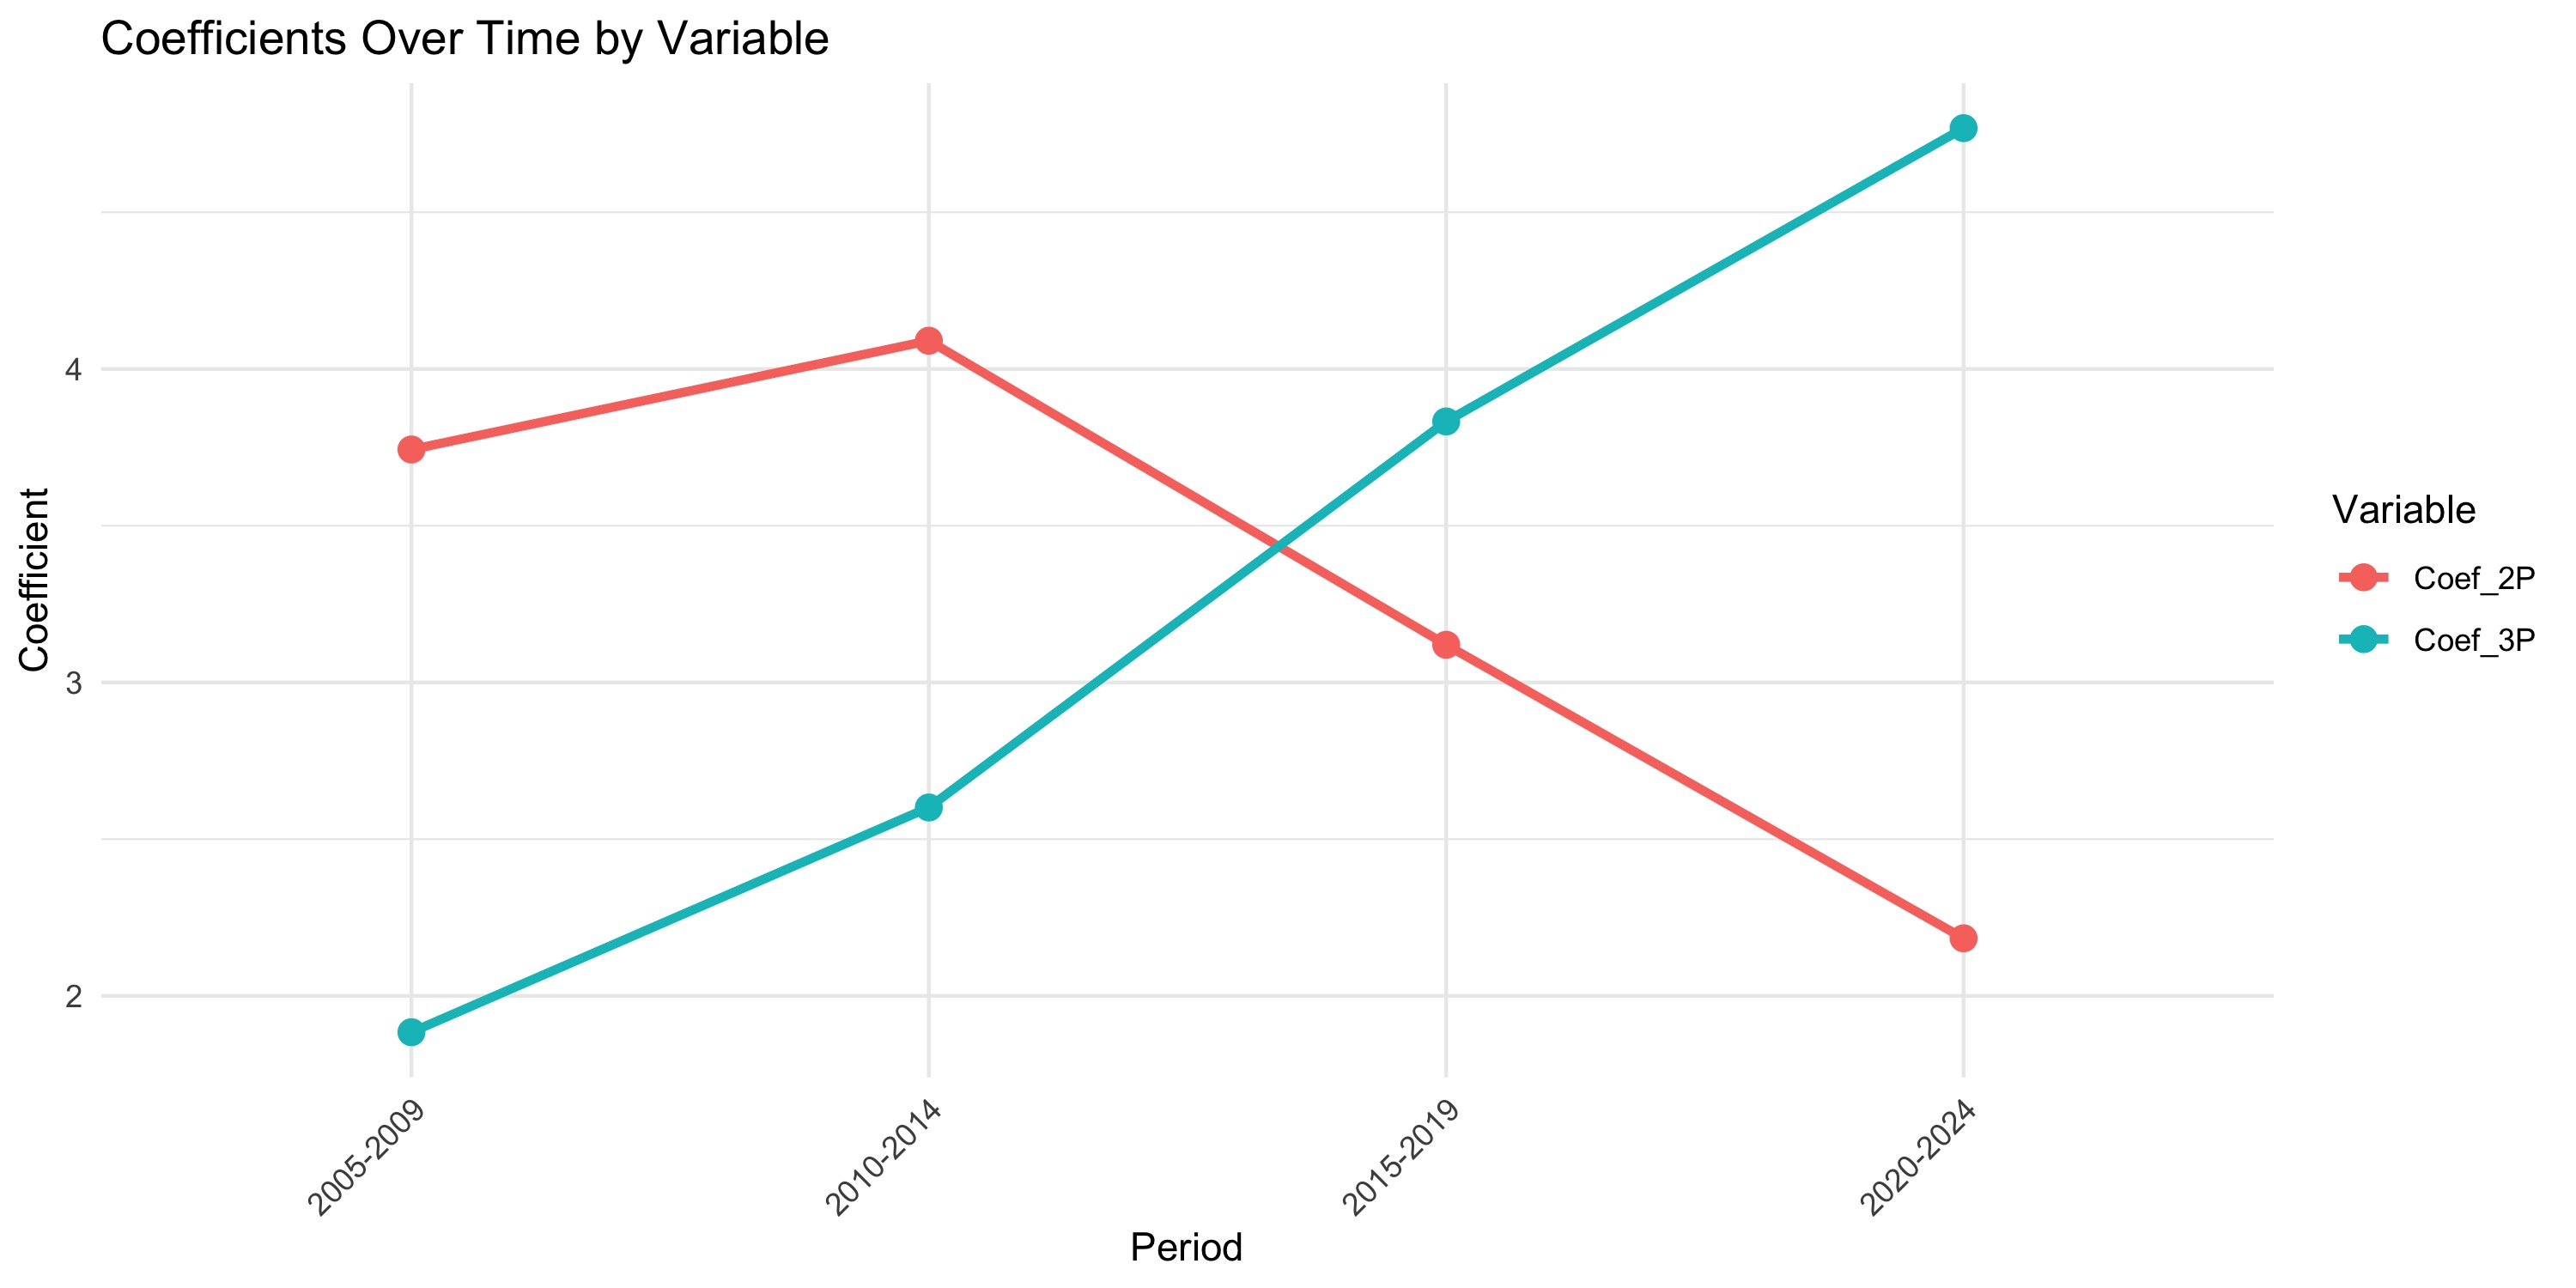
\includegraphics[width=0.7\textwidth]{figure/Coefficients Over Time by Variable.jpg} 
    \caption{Trends in Estimated Coefficients for 3P\% (Coef\_3P) and 2P\% (Coef\_2P) from Period-Specific Regressions (WinRate ~ 3P\% + 2P\% + 3P\_ratio).}
    \label{fig:coefficients_trends}
\end{figure}

\subsection{Interaction Model: Quantifying the Shift}
To formally test our thesis that the association between shooting metrics and win rate significantly differs between eras, we fit the interaction model using combined data from the 2005-2009 (Era=0) and 2020-2024 (Era=1) periods, as specified in the Methods section. The results from this model, based on the R output provided, are summarized in Table \ref{tab:interaction_summary_R}.

% --- START: Interaction Model Summary Table based on R output image ---
\begin{table}[htbp]
\centering
\caption{Summary of Interaction Model Results (Response: WinRate, based on R output)}
\label{tab:interaction_summary_R}
% Note: Using booktabs package for better table formatting
\begin{tabular}{lrrrr}
\toprule
Predictor & Estimate & Std. Error & t value & Pr(>|t|) \\
\midrule
(Intercept) & -2.0312 & 0.2812 & -7.224 & 4.41e-12 *** \\ 
X3P. & 1.8842 & 0.5918 & 3.184 & 0.001610 ** \\ 
X2P. & 3.7431 & 0.5910 & 6.334 & 9.02e-10 *** \\ 
X3P\_ratio & 0.2650 & 0.2359 & 1.123 & 0.262187 \\ 
Era (1 = 2020-24) & -0.2905 & 0.3879 & -0.749 & 0.454448 \\ 
**X3P.:Era** & **2.8842** & **0.8641** & **3.338** & **0.000954 *** \\** X2P.:Era & -1.5594 & 0.7616 & -2.047 & 0.041509 * \\ 
X3P\_ratio:Era & -0.4431 & 0.3434 & -1.290 & 0.197976 \\ 
\midrule
\multicolumn{5}{l}{\textit{Signif. codes: 0 '***' 0.001 '**' 0.01 '*' 0.05 '.' 0.1 ' ' 1}} \\
\multicolumn{5}{l}{Residual standard error: 0.1123 on 292 degrees of freedom} \\ 
\multicolumn{5}{l}{Multiple R-squared: 0.4301, Adj. R-squared: 0.4165} \\ 
\multicolumn{5}{l}{F-statistic: 31.49 on 7 and 292 DF, p-value: < 2.2e-16} \\ 
\bottomrule
\end{tabular}
\end{table}
% --- END: Interaction Model Summary Table ---

The results presented in Table \ref{tab:interaction_summary_R} provide the key statistical evidence for our study. 
Our primary interest lies in the interaction term between three-point percentage and era, denoted as \texttt{X3P.:Era} in the model output. 
This term's coefficient is estimated at approximately 2.8842, and it is highly statistically significant (p $\approx$ 0.000954, indicated by '***'). 
This positive and significant interaction coefficient confirms our central hypothesis: the statistical association between a team's three-point percentage (\texttt{X3P.}) and its win rate (\texttt{WinRate}) is significantly stronger in the more recent era (2020-2024, when Era=1) compared to the baseline era (2005-2009, when Era=0). 
Specifically, the model estimates that for every one percentage point increase in \texttt{X3P.}, the associated increase in \texttt{WinRate} is about 2.88 points higher in the 2020-2024 era than it was in the 2005-2009 era, holding other predictors constant.

Looking at the main effects in the baseline era (Era=0), both the three-point percentage \texttt{X3P.} (Coefficient $\approx$ 1.88, p $\approx$ 0.0016) and the two-point percentage \texttt{X2P.} (Coef. $\approx$ 3.74, p $<$ 0.001) show a statistically significant positive association with \texttt{WinRate}. 
The interaction term \texttt{X2P.:Era} (Coef. $\approx$ -1.56, p $\approx$ 0.042) is negative and statistically significant at the 0.05 level. This suggests that the positive association for two-point percentage weakened in the later era, aligning with the descriptive trends observed earlier. 
Neither the three-point attempt rate (variable \texttt{X3P\_ratio}) nor its interaction with era (\texttt{X3P\_ratio:Era}), nor the main effect of \texttt{Era} itself, showed a statistically significant association with \texttt{WinRate} in this model. 
The overall model demonstrates a reasonable fit (Adjusted R-squared $\approx$ 0.4165) and is statistically significant (F-statistic p-value $<$ 2.2e-16). 
In summary, the highly significant interaction for \texttt{X3P.:Era} provides strong statistical support for our thesis regarding the substantially increased importance associated with three-point shooting efficiency in the modern NBA.

\subsection{Model Diagnostics}
% Word Count: Approx. 100-150 words

Finally, we assessed the validity of the assumptions underlying the OLS regression for our final interaction model (results in Table \ref{tab:interaction_summary_R}). The standard diagnostic plots are presented in Figure \ref{fig:diagnostic_plots}. 

% IMPORTANT: Ensure this figure path points to the DIAGNOSTIC PLOTS FOR THE R INTERACTION MODEL
\begin{figure}[htbp] 
    \centering
    % Assuming the plots on Page 5 of the PDF *are* for this R model. If not, replace the file path.
    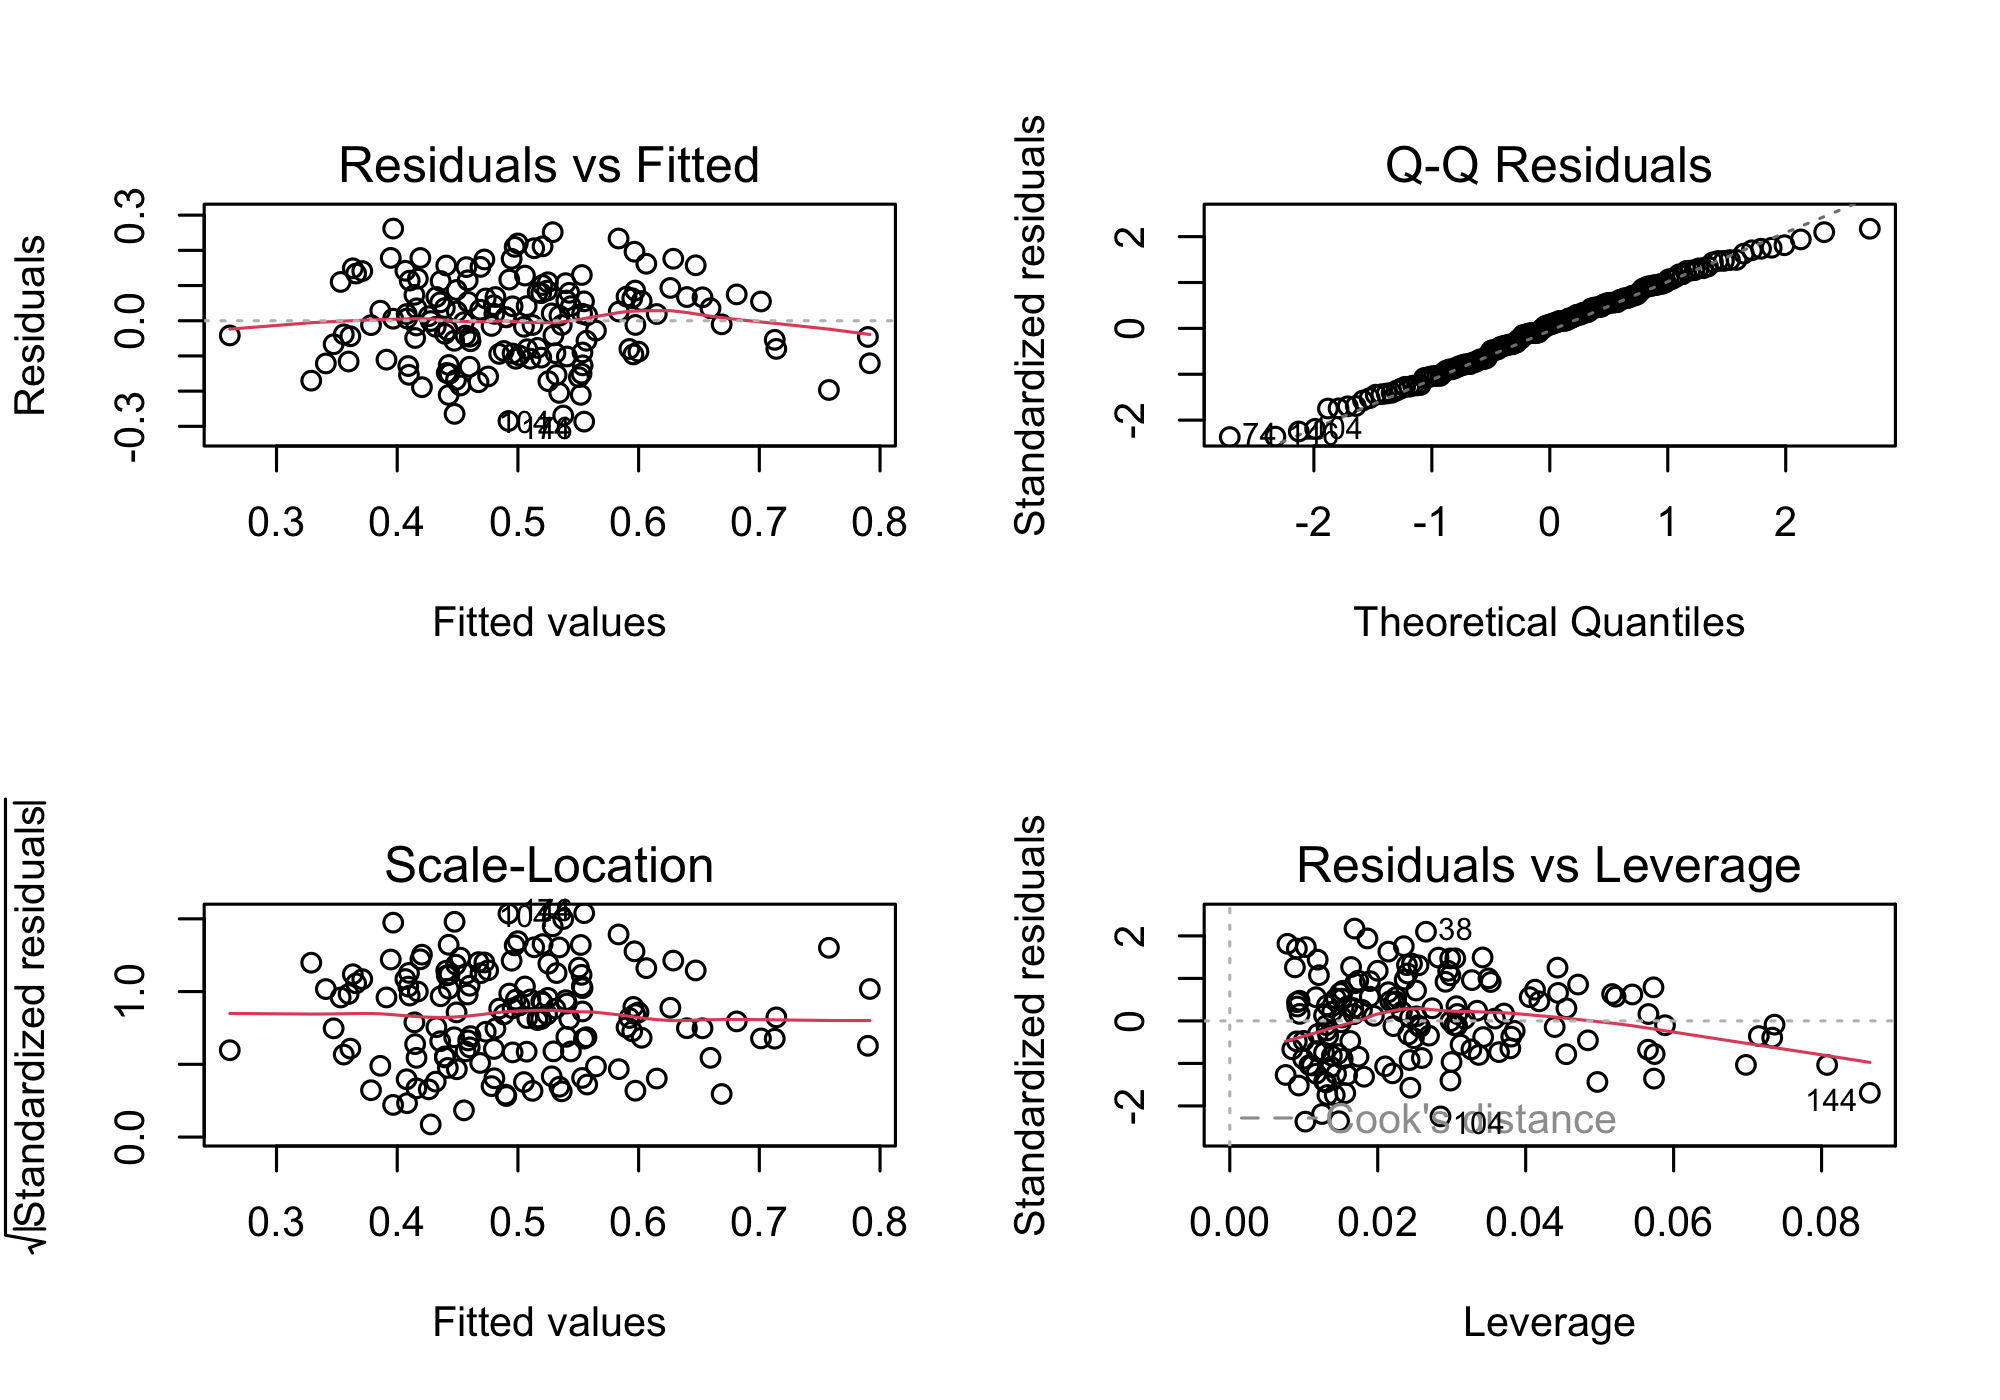
\includegraphics[width=0.9\textwidth]{figure/diagnostic_plots_mydf_2005_2009.png}
    \caption{Diagnostic Plots for the Final Interaction Model (R Output).} 
    \label{fig:diagnostic_plots}
\end{figure}

The 'Residuals vs Fitted' plot displays residuals scattered around the zero line without a clear funnel shape or curve, suggesting the assumptions of linearity and constant variance (homoscedasticity) are generally met. The 'Normal Q-Q' plot shows points lying reasonably close to the diagonal line, indicating that the residuals are approximately normally distributed, which supports the reliability of our significance tests. The 'Scale-Location' plot further checks for homoscedasticity, and the spread appears relatively constant across fitted values. The 'Residuals vs Leverage' plot helps identify influential cases; based on this plot (examine your specific plot for points exceeding Cook's distance contours), no single observation appears to exert undue influence on the model estimates. Therefore, based on these visual checks, the model assumptions seem adequately satisfied, supporting the robustness of our findings from the interaction model.

%----------------------------------------------------------------------------------------
% End of Results Section
%----------------------------------------------------------------------------------------

%----------------------------------------------------------------------------------------
% Conclusion Section
%----------------------------------------------------------------------------------------

\section{Conclusion} % Main Section Title

\subsection{Summary of Findings in Relation to Thesis} % Sub-section 4.1
% Word Count: Approx. 100 words
This project investigated the evolving statistical relationship between shooting strategy, particularly three-point shooting, and team success in the NBA over approximately two decades. We aimed to statistically assess the narrative of a "Three-Point Era." Our analysis leads us to affirm our central thesis statement: 
Using data from the 2005-2009 and 2020-2024 NBA regular seasons (source: NBA API), we find the statistical association between three-point percentage (3P\%) and win rate differs significantly between these periods: NBA team-seasons in the 2020-2024 period with higher 3P\% also have statistically significant higher win rates, while NBA team-seasons in the 2005-2009 period did not have statistically significant higher win rates, even after controlling for two-point efficiency and shot selection proportions.
The primary evidence supporting this thesis comes from our interaction model analysis (Table \ref{tab:interaction_summary_R}), which revealed a highly statistically significant interaction term between three-point percentage and era (`Era:X3P.`). This finding was further supported by descriptive trends showing a strengthening association for 3P\% and a weakening one for 2P\% over time (Figure \ref{fig:coefficients_trends}).

\subsection{Interpretation and Implications} % Sub-section 4.2
The significant interaction term (`Era:X3P.`) indicates that the strength of the positive statistical association between three-point percentage and win rate has substantially increased from the 2005-2009 period to the 2020-2024 period. Our model estimated this increase in association strength to be approximately 2.88 points (referencing Table \ref{tab:interaction_summary_R}). This provides quantitative, structural evidence consistent with the popular notion of an NBA "Three-Point Era." It suggests that characteristics related to high-efficiency three-point shooting are much more strongly associated with winning in today's league compared to 15-20 years ago. 
While our observational study design prevents definitive causal claims, the statistically significant *change* in this association, detected through the interaction model, offers a result consistent with the hypothesis that the underlying strategic value or contribution of efficient three-point shooting to winning has genuinely increased. It suggests that optimizing for three-point efficiency yields a stronger association with success now than it did previously.

\subsection{Limitations of the Analysis} % Sub-section 4.3
It is crucial to acknowledge the limitations inherent in this study. The most significant limitation stems from the use of observational data. While we found a significant change in statistical association, we cannot definitively conclude a causal relationship between increased 3P\% efficiency and increased win rates. Correlation does not imply causation. 
A primary concern is the potential for **unobserved confounding variables**. Many factors beyond the shooting metrics included in our model could influence both a team's strategic choices (like emphasizing threes) and its overall success (win rate). Examples include:
\begin{itemize}
    \item \textbf{Rule Changes:} Modifications to defensive rules (e.g., hand-checking elimination, defensive three seconds) over the analyzed period likely affected offensive and defensive strategies.
    \item \textbf{Coaching Philosophy and Quality:} Different coaches employ varying strategies, and overall coaching quality impacts team success independently of specific shooting metrics. The league-wide adoption of analytics also plays a role here.
    \item \textbf{Player Skill Evolution & Specific Stars:} The general skill level of shooters may have increased, and the presence of generational talents (like Stephen Curry, who dramatically influenced offensive schemes) is not directly accounted for in our team-level aggregate data.
    \item \textbf{Other Team Factors:} Unaccounted factors like specific player injuries during a season, variations in strength of schedule, changes in league pace, or evolving defensive schemes employed against teams could all confound the observed relationships.
\end{itemize}
While we controlled for 2P\% and shot selection proportions, the potential for residual confounding from these and other unmeasured variables remains. Other limitations include potential measurement errors in the API data, the specific choice of 5-year periods for trend analysis, and the inherent assumptions of the linear regression model (linearity, independence, normality, homoscedasticity), which may only be approximately met.

\subsection{Future Research} % Sub-section 4.4
Based on our findings and limitations, several avenues for future research emerge. Incorporating additional control variables, such as team defensive ratings, offensive/defensive rebound percentages, pace, or perhaps team fixed effects, could help mitigate confounding concerns. Analyzing player-level data could provide insights into individual contributions and skill changes. Examining playoff data separately might reveal if these associations hold under higher-stakes conditions. Finally, exploring more advanced statistical methods designed for causal inference with observational data (e.g., instrumental variables, if suitable instruments could be identified) might offer further insights, although likely challenging in this context.

\subsection{Concluding Remarks} % Sub-section 4.5
In conclusion, this project provides robust statistical evidence, primarily through the analysis of interaction effects, demonstrating a significant strengthening in the association between three-point shooting efficiency and team success in the NBA over the last two decades, quantitatively supporting the narrative of a "Three-Point Era."

%----------------------------------------------------------------------------------------
% End of Conclusion Section
%----------------------------------------------------------------------------------------
%----------------------------------------------------------------------------------------
% References
%----------------------------------------------------------------------------------------

\newpage % Includes a new page
\pagenumbering{roman} % Changes page numbering to roman page numbers
%\bibliography{literature}

\bibliography{literature.bib} % Add the filename of your bibliography
\bibliographystyle{apsr} % Defines your bibliography style

%----------------------------------------------------------------------------------------
% Appendix
%----------------------------------------------------------------------------------------

\newpage
\pagenumbering{roman} % Changes page numbering to roman page numbers

\section*{Appendix}

% For citing, please see this sheet: http://merkel.texture.rocks/Latex/natbib.php

% %----------------------------------------------------------------------------------------
% % Appendix
% %----------------------------------------------------------------------------------------
% \newpage % Includes a new page
% \section*{Appendix} % Stars disable section numbers
% % \appendix % Uncomment if you want to add an "automatic" appendix
% \pagenumbering{Roman} % Changes page numbering to Roman page numbers

% \blindtext % Adds some blind text

% %----------------------------------------------------------------------------------------
% % Declaration
% %----------------------------------------------------------------------------------------
% \newpage % Includes a page break
% \thispagestyle{empty} % Leaves the page style empty (no page number, no header, no footer)
% \section*{Statutory Declaration} % Stars disable section numbers

% \begin{otherlanguage}{german}
% Hiermit versichere ich, dass diese Arbeit von mir pers\"{o}nlich verfasst ist und dass ich keinerlei fremde Hilfe in Anspruch genommen habe. Ebenso versichere ich, dass diese Arbeit oder Teile daraus weder von mir selbst noch von anderen als Leistungsnachweise andernorts eingereicht wurden. W\"{o}rtliche oder sinngem\"{a}{\ss}e \"{U}bernahmen aus anderen Schriften und Ver\"{o}ffentlichungen in gedruckter oder elektronischer Form sind gekennzeichnet. S\"{a}mtliche Sekund\"{a}rliteratur und sonstige Quellen sind nachgewiesen und in der Bibliographie aufgef\"{u}hrt. Das Gleiche gilt f\"{u}r graphische Darstellungen und Bilder sowie f\"{u}r alle Internet-Quellen. Ich bin ferner damit einverstanden, dass meine Arbeit zum Zwecke eines Plagiatsabgleichs in elektronischer Form anonymisiert versendet und gespeichert werden kann. Mir ist bekannt, dass von der Korrektur der Arbeit abgesehen und die Pr\"{u}fungsleistung mit nicht ausreichend bewertet werden kann, wenn die Erkl\"{a}rung nicht erteilt wird.
% \end{otherlanguage}

% \vspace*{1in} % Adds extra space between two paragraphs

% \noindent I hereby declare that the paper presented is my own work and that I have not called upon the help of a third party. In addition, I affirm that neither I nor anybody else has submitted this paper or parts of it to obtain credits elsewhere before. I have clearly marked and acknowledged all quotations or references that have been taken from the works of others. All secondary literature and other sources are marked and listed in the bibliography. The same applies to all charts, diagrams and illustrations as well as to all Internet resources. Moreover, I consent to my paper being electronically stored and sent anonymously in order to be checked for plagiarism. I am aware that the paper cannot be evaluated and may be graded ``failed'' (``nicht ausreichend'') if the declaration is not made.\\

% %\vspace*{1in} % Adds extra space

% % Add field for signature, date, and place
% \hfill \signature{} 


% %---------------------------------------------------------------------------------

\end{document}
